%FIXME still fragile as hell

\centering

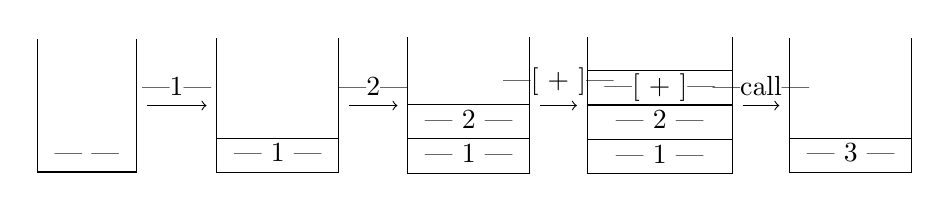
\begin{tikzpicture}[node distance=0.2\linewidth]
  \node (a) {
    \begin{tabular}{|c|}
      \texttt{~}         \\
      \texttt{~}         \\
      \texttt{~}         \\
      \inlinecode|     | \\ \hline
    \end{tabular}
  };

  \node (b) [right of=a] {
    \begin{tabular}{|c|}
      \texttt{~}         \\
      \texttt{~}         \\
      \texttt{~}         \\ \hline
      \inlinecode|  1  | \\ \hline
    \end{tabular}
  };

  \node (c) [right of=b] {
    \begin{tabular}{|c|}
      \texttt{~}         \\
      \texttt{~}         \\ \hline
      \inlinecode|  2  | \\ \hline
      \inlinecode|  1  | \\ \hline
    \end{tabular}
  };

  \node (d) [right of=c] {
    \begin{tabular}{|c|}
      \texttt{~}        \\ \hline
      \inlinecode|[ + ]| \\ \hline
      \inlinecode|  2  | \\ \hline
      \inlinecode|  1  | \\ \hline
    \end{tabular}
  };

  \node (e) [right of=d] {
    \begin{tabular}{|c|}
      \texttt{~}        \\
      \texttt{~}        \\
      \texttt{~}        \\ \hline
      \inlinecode|  3  | \\ \hline
    \end{tabular}
  };


  \path[->] (a) edge node [above] {\inlinecode|1|}     (b)
            (b) edge node [above] {\inlinecode|2|}     (c)
            (c) edge node [above] {\inlinecode|[ + ]|} (d)
            (d) edge node [above] {\inlinecode|call|}  (e);
\end{tikzpicture}

\caption{Quotations}
